\section{Empirical Results}

We design experiments to explore the following research questions. 

\begin{itemize}[leftmargin=*]
    % calculate the distances between model pairs using L2/abs_mean/abs_max/1-cosine
    \item \textbf{Measurement Evaluation (RQ1)}: How do different measurement metrics affect the effectiveness of LLM lineage detection?
    % \item \textbf{Lineage Type Evaluation (RQ2)}: How do different lineage types contribute to the performance of LLM lineage detection?
    % calculate the distances between model pairs using mlp/k/q/v/o
    \item \textbf{Layers in Transformer Block Evaluation (RQ2)}: How do different model layers influence the effectiveness of LLM lineage detection?
    % using different graph algorithms to detect lineage, like Chu-Liu-Edmonds algorithm...
    \item \textbf{Graph Algorithms Evaluation (RQ3)}: How do different graph algorithms influence the effectiveness of LLM lineage detection?
    % \item \textbf{State-of-the-art Evaluation (RQ4)}: How do different model layers influence the effectiveness of LLM lineage detection?
    % analyze why existing methods fail to detect lineage
    \item \textbf{Failure Analysis (RQ4)}: Why do existing methods fail to detect lineage?
\end{itemize}

\subsection{RQ1}

% put graph here, below is a demo.
% \begin{figure*}[!t]
%     \centering
%     \begin{subfigure}{0.44\linewidth}
%         \centering
%         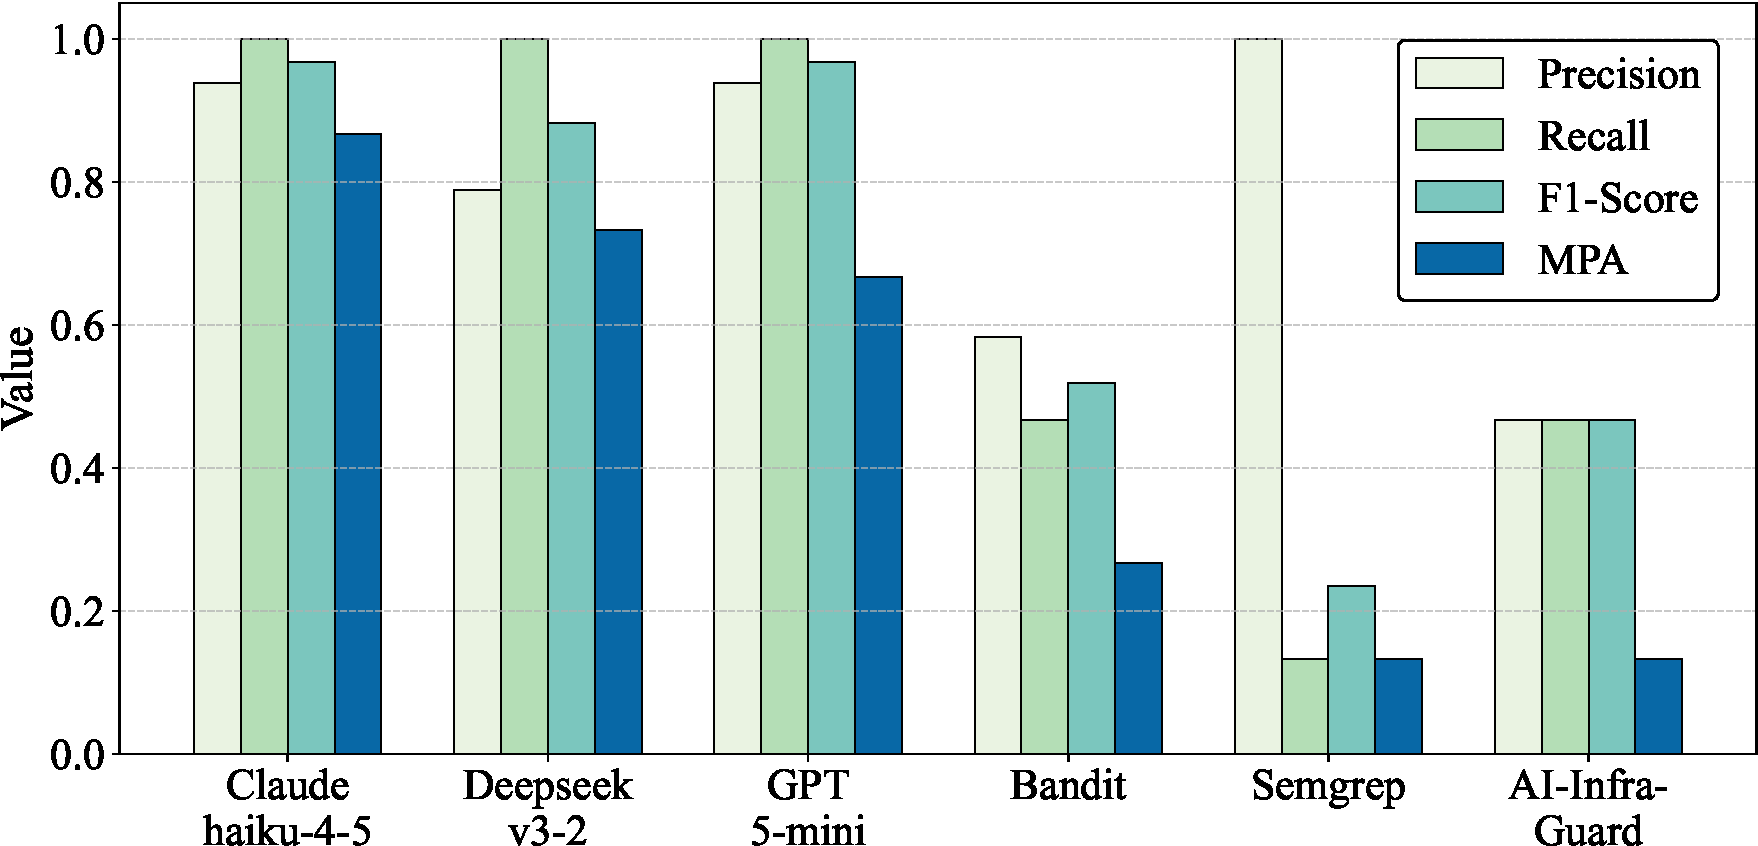
\includegraphics[width=\linewidth]{fig/RCE.pdf}
%            \vspace{-9pt}
%         \caption{Remote Code Execution}
%         \label{fig:sub1}
%     \end{subfigure}%
%     \begin{subfigure}{0.44\linewidth}
%         \centering
%         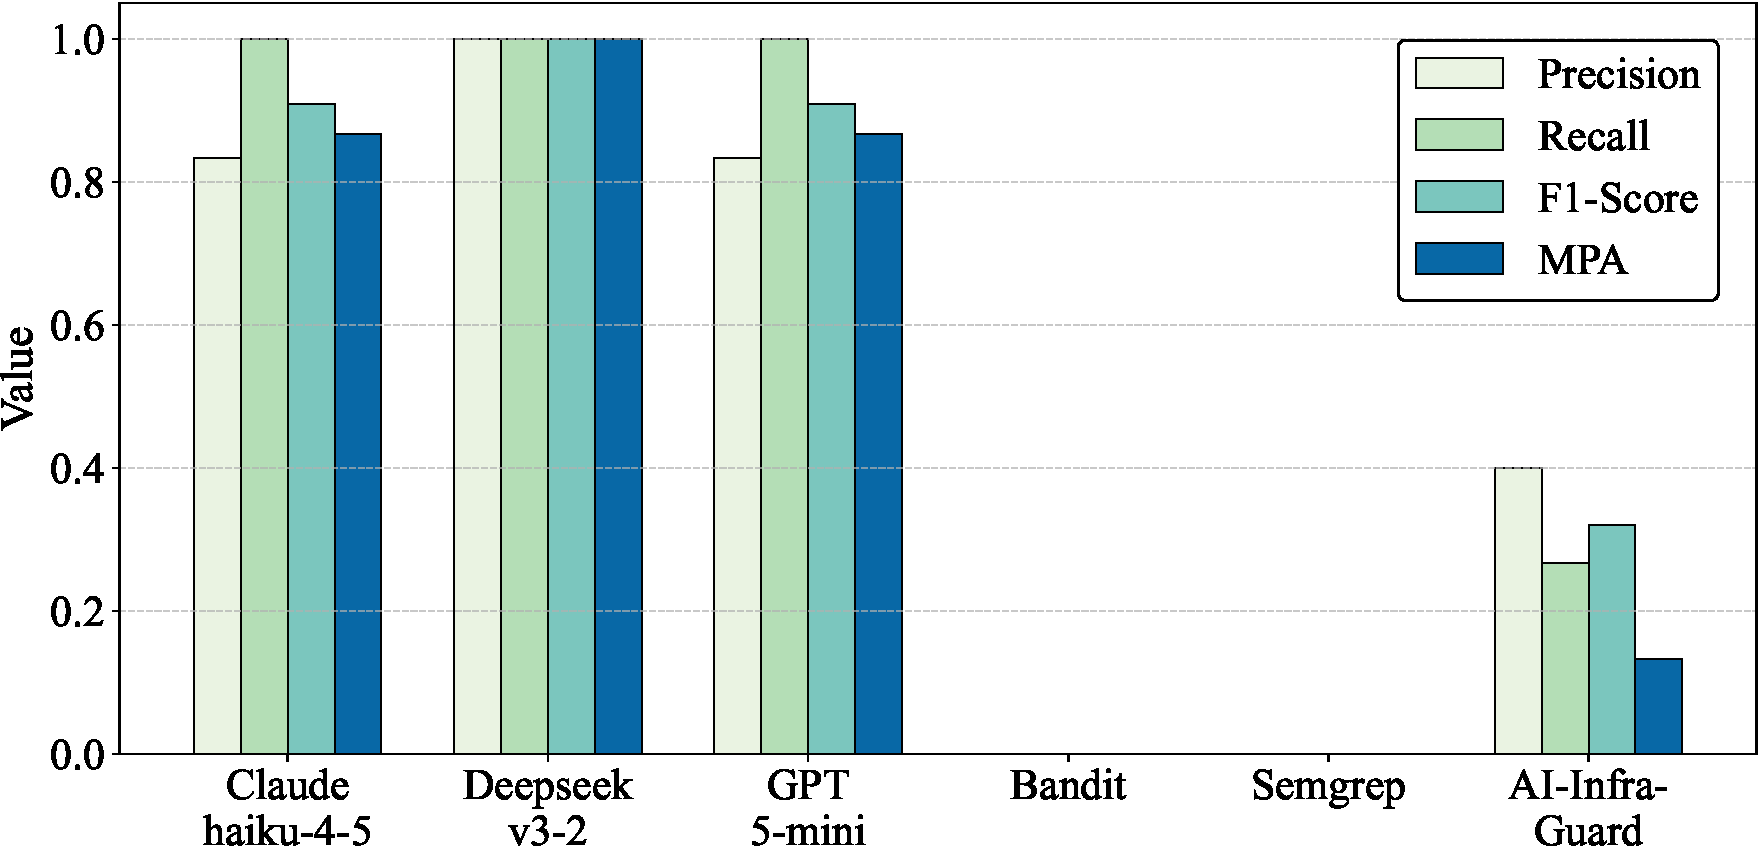
\includegraphics[width=\linewidth]{fig/SID.pdf}
%            \vspace{-9pt}
%         \caption{Sensitive Information Disclosure}
%         \label{fig:sub2}
%     \end{subfigure}%
%     \hfill
%      \begin{subfigure}{0.44\linewidth}
%         \centering
%         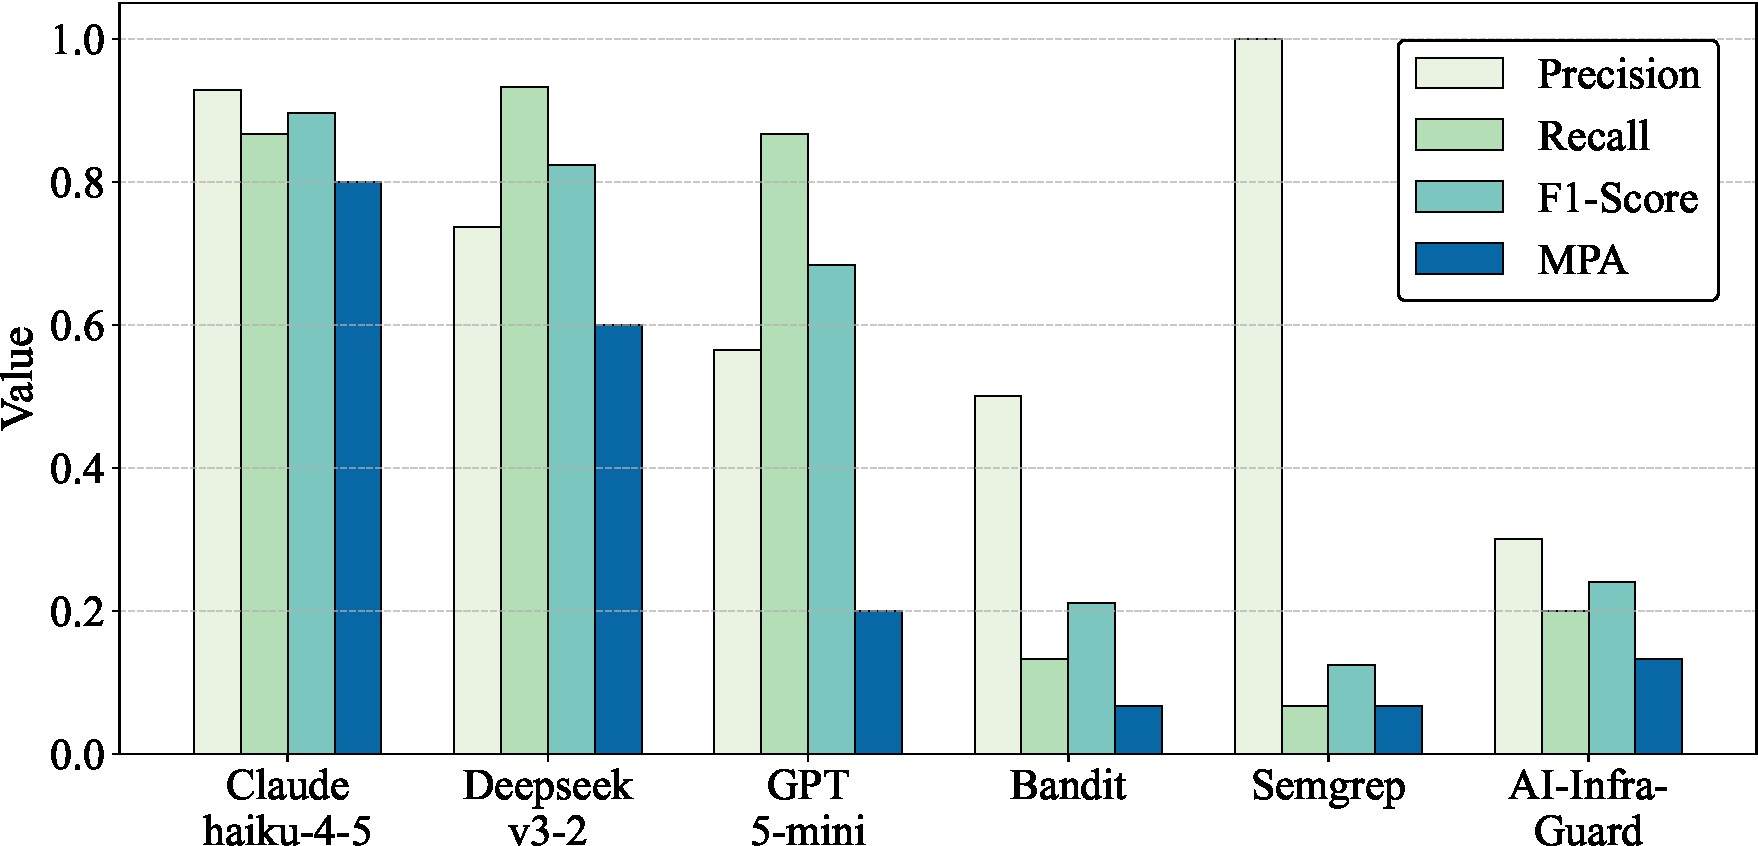
\includegraphics[width=\linewidth]{fig/IFO.pdf}
%             \vspace{-9pt}
%         \caption{Insecure File Operation}
%         \label{fig:sub3}
%     \end{subfigure}%
%      \begin{subfigure}{0.44\linewidth}
%         \centering
%         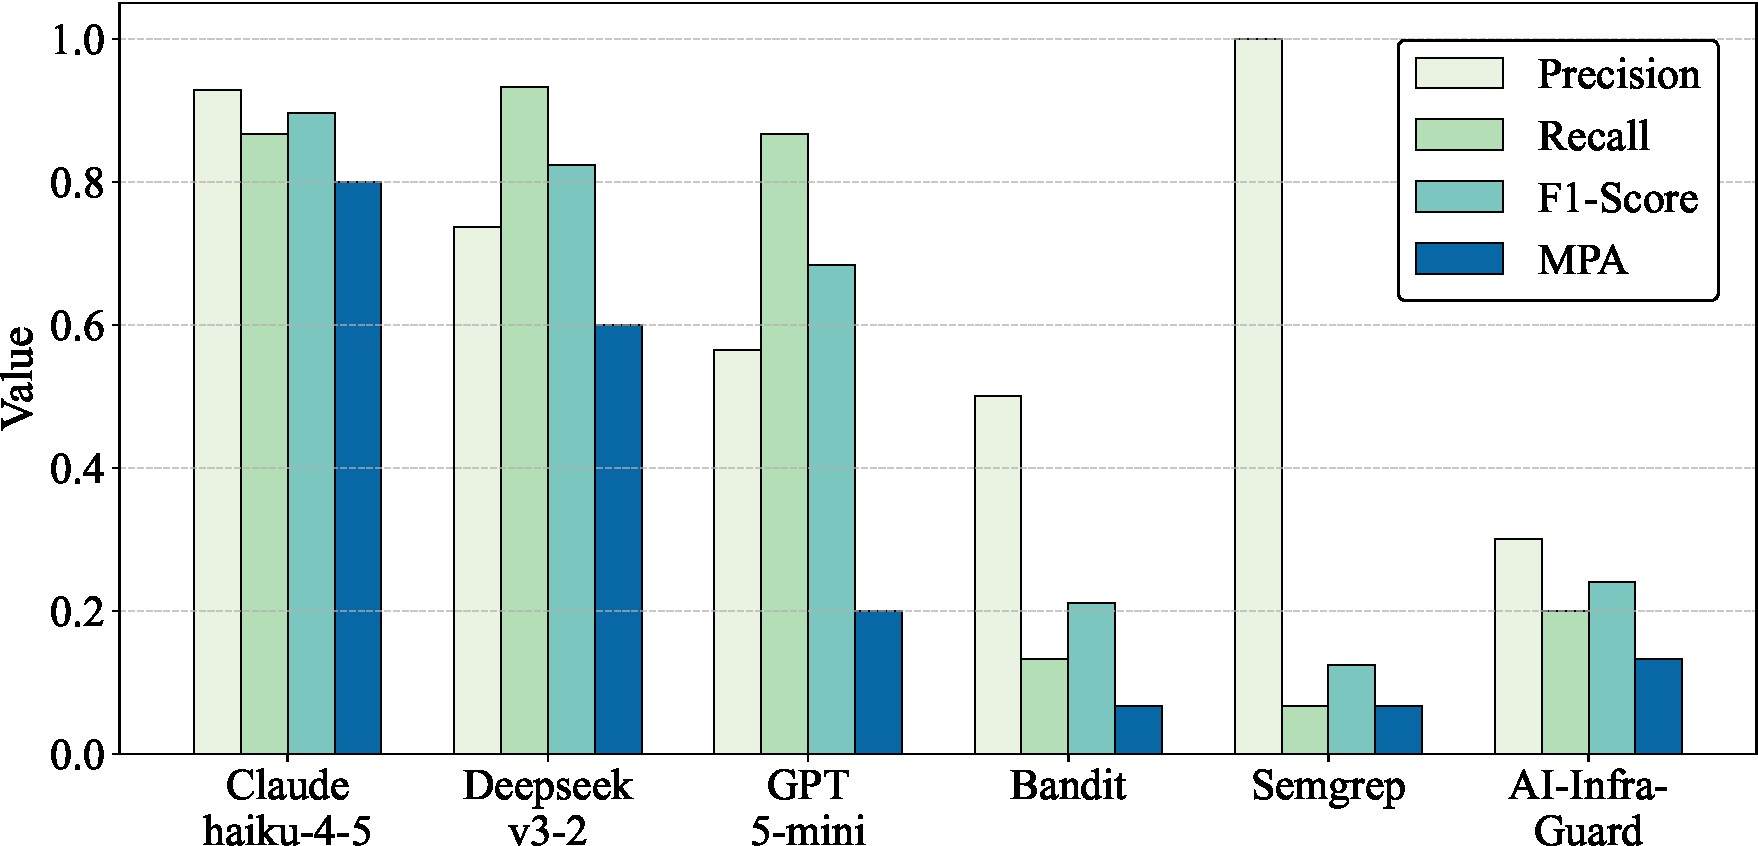
\includegraphics[width=\linewidth]{fig/IFO.pdf}
%            \vspace{-9pt}
%         \caption{SQL Injection}
%         \label{fig:sub4}
%     \end{subfigure}%
%     \vspace{-10pt}
%     \caption{Experimental Results w.r.t MCP Tool Vulnerability Types}
%     \label{fig:eva2}
% \end{figure*}

\begin{table}[t]
    \caption{Lineage Detection Accuracy (\%) w.r.t. Different Measurement Metrics (RQ1)}
    \label{tab:rq1-metrics-comp}
    \centering
    \resizebox{\columnwidth}{!}{
        \begin{tabular}{@{}lcccccc@{}}
            \toprule
            \textbf{Direction Method} & \textbf{L2} & \textbf{Cos.} & \textbf{Abs Mean} & \textbf{Abs Max} & \textbf{Sparse Abs.} & \textbf{Sparse Rel.} \\ 
            \midrule
            kurtosis & 72.1 & 65.4 & 58.9 & 44.2 & ... \\
            timestamp & 72.1 & 65.4 & 58.9 & 44.2 & ... \\
            \bottomrule
        \end{tabular}
    }
\end{table}

\subsection{RQ2}

% figures show different layers' contribution to L2 distance
\begin{figure}[t]
    \centering
    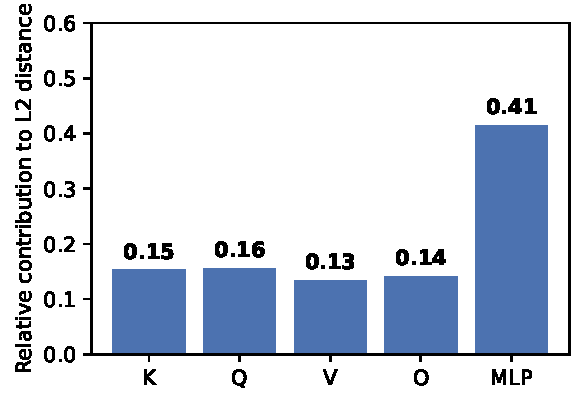
\includegraphics[width=\columnwidth]{fig/rq2_l2_layer_contrib.pdf}
    \caption{Contribution of different transformer block components (K/Q/V/O/MLP) to L2 distance (RQ2).}
    \label{fig:rq2-l2-layer-contrib}
\end{figure}

% heatmap show different layers' contribution to tree construction accuracy
\begin{figure}[t]
    \centering
    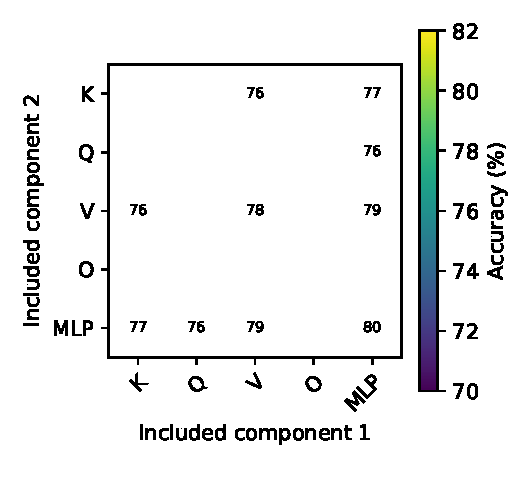
\includegraphics[width=\columnwidth]{fig/rq2_layer_combo_heatmap.pdf}
    \caption{Accuracy of lineage detection with different combinations of transformer block components (RQ2).}
    \label{fig:rq2-layer-combo-heatmap}
\end{figure}

\subsection{RQ3}

% except for MoTHer, we use timestamp as direction method for other graph algorithms
\begin{table}[t]
    \caption{Lineage Detection Accuracy (\%) w.r.t. Different Graph Algorithms (RQ3). Except for MoTHer, we use timestamp as the direction method for other graph algorithms.}
    \label{tab:rq4-ablation}
    \centering
    \begin{tabular}{@{}lcc@{}}
        \toprule
        \textbf{Graph Algorithm} & \textbf{Accuracy (\%)} \\ \midrule
        Baseline (MoTHer) & - & - \\
        + MoTHer-Timestamp & - & - \\
        + Hard-Constraint & - & - \\
        + Undirected-Mst  & - & - \\ 
        + atlas\_snake\_fan & - & - \\
        \bottomrule
    \end{tabular}
\end{table}

\subsection{RQ4}

% sector graph error analysis of siblings-edge & grandparent-child-edge portion w. timestamp & parent-child-inverse-edge w/o. timestamp
\begin{figure}[t]
    \centering
    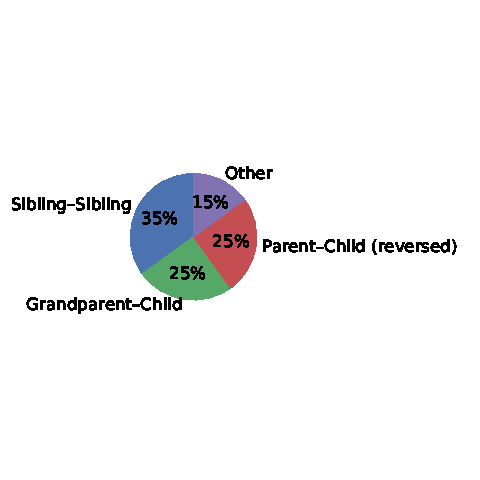
\includegraphics[width=\columnwidth]{fig/rq4_error_edge_pie.pdf}
    \caption{Proportion of different types of erroneous edges in the constructed lineage graph (RQ4).}
    \label{fig:rq4-error-pie}
\end{figure}

% a example of case study of ...
\begin{figure}[t]
    \centering
    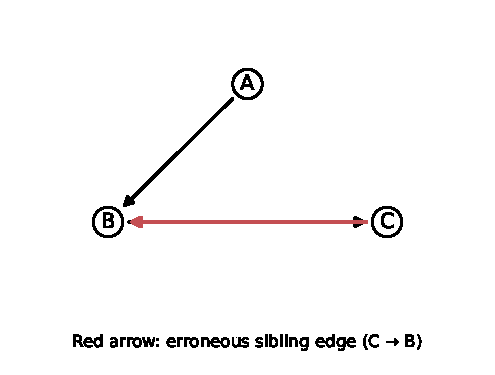
\includegraphics[width=\columnwidth]{fig/rq4_error_case_study.pdf}
    \caption{Case study illustrating erroneous edges in the constructed lineage graph (RQ4).}
    \label{fig:rq4-error-case}
\end{figure}